\documentclass[crop,tikz]{standalone}

\begin{document}
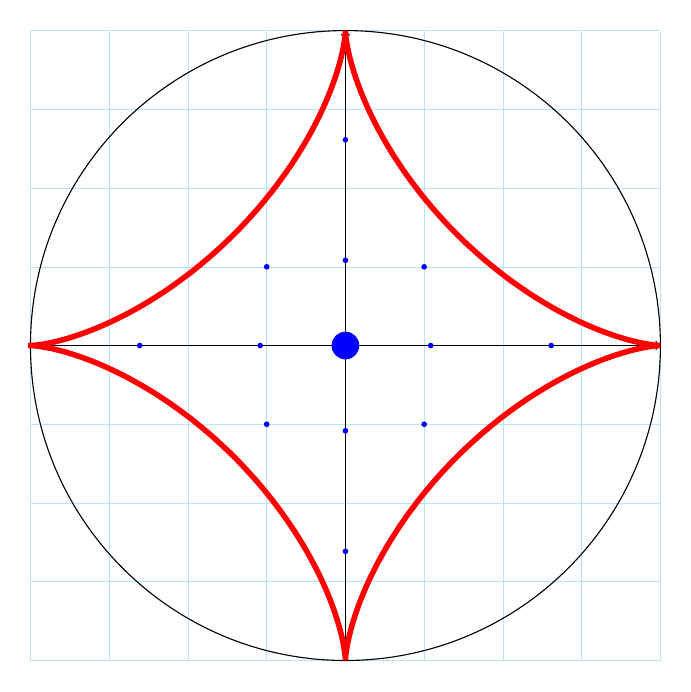
\begin{tikzpicture}
\def\a{1} \def\b{4} \def\scale{1}
\draw[cyan!30,very thin] ({-\b*\scale},{-\b*\scale}) grid ({\b*\scale},{\b*\scale});
\draw[->] ({-\b*\scale},0) -- ({\b*\scale},0);
\draw[->] (0,{-\b*\scale}) -- (0,{\b*\scale});
\draw (0,0) circle ({\b*\scale});
\draw[line width=2pt,red] plot[samples=100,domain=0:\a*360,smooth,variable=\t] ({\scale*((\b-\a)*cos(\t)+\a*cos((\b-\a)*\t/\a)},{\scale*((\b-\a)*sin(\t)-\a*sin((\b-\a)*\t/\a)});

\draw[blue,fill=blue] (-2.613125929752753,-0.0) circle (4*0.200000000000000pt);
\draw[blue,fill=blue] (1.082392200292394,-0.0) circle (4*0.200000000000000pt);
\draw[blue,fill=blue] (-1.0,1.0) circle (4*0.200000000000000pt);
\draw[blue,fill=blue] (-0.0,2.613125929752753) circle (4*0.200000000000000pt);
\draw[blue,fill=blue] (0.0,1.082392200292394) circle (4*0.200000000000000pt);
\draw[blue,fill=blue] (-1.0,-1.0) circle (4*0.200000000000000pt);
\draw[blue,fill=blue] (0.0,0.0) circle (4*1.20000000000000pt);
\draw[blue,fill=blue] (-0.0,-1.082392200292394) circle (4*0.200000000000000pt);
\draw[blue,fill=blue] (1.0,-1.0) circle (4*0.200000000000000pt);
\draw[blue,fill=blue] (-1.082392200292394,0.0) circle (4*0.200000000000000pt);
\draw[blue,fill=blue] (0.0,-2.613125929752753) circle (4*0.200000000000000pt);
\draw[blue,fill=blue] (1.0,1.0) circle (4*0.200000000000000pt);
\draw[blue,fill=blue] (2.613125929752753,0.0) circle (4*0.200000000000000pt);
\end{tikzpicture}

\end{document}